\documentclass{standalone}
\usepackage{tikz}
\usetikzlibrary{patterns, positioning}
\usepackage[sfdefault]{ClearSans} %% option 'sfdefault' activates Clear Sans as the default text font
\usepackage[T1]{fontenc}

\begin{document}
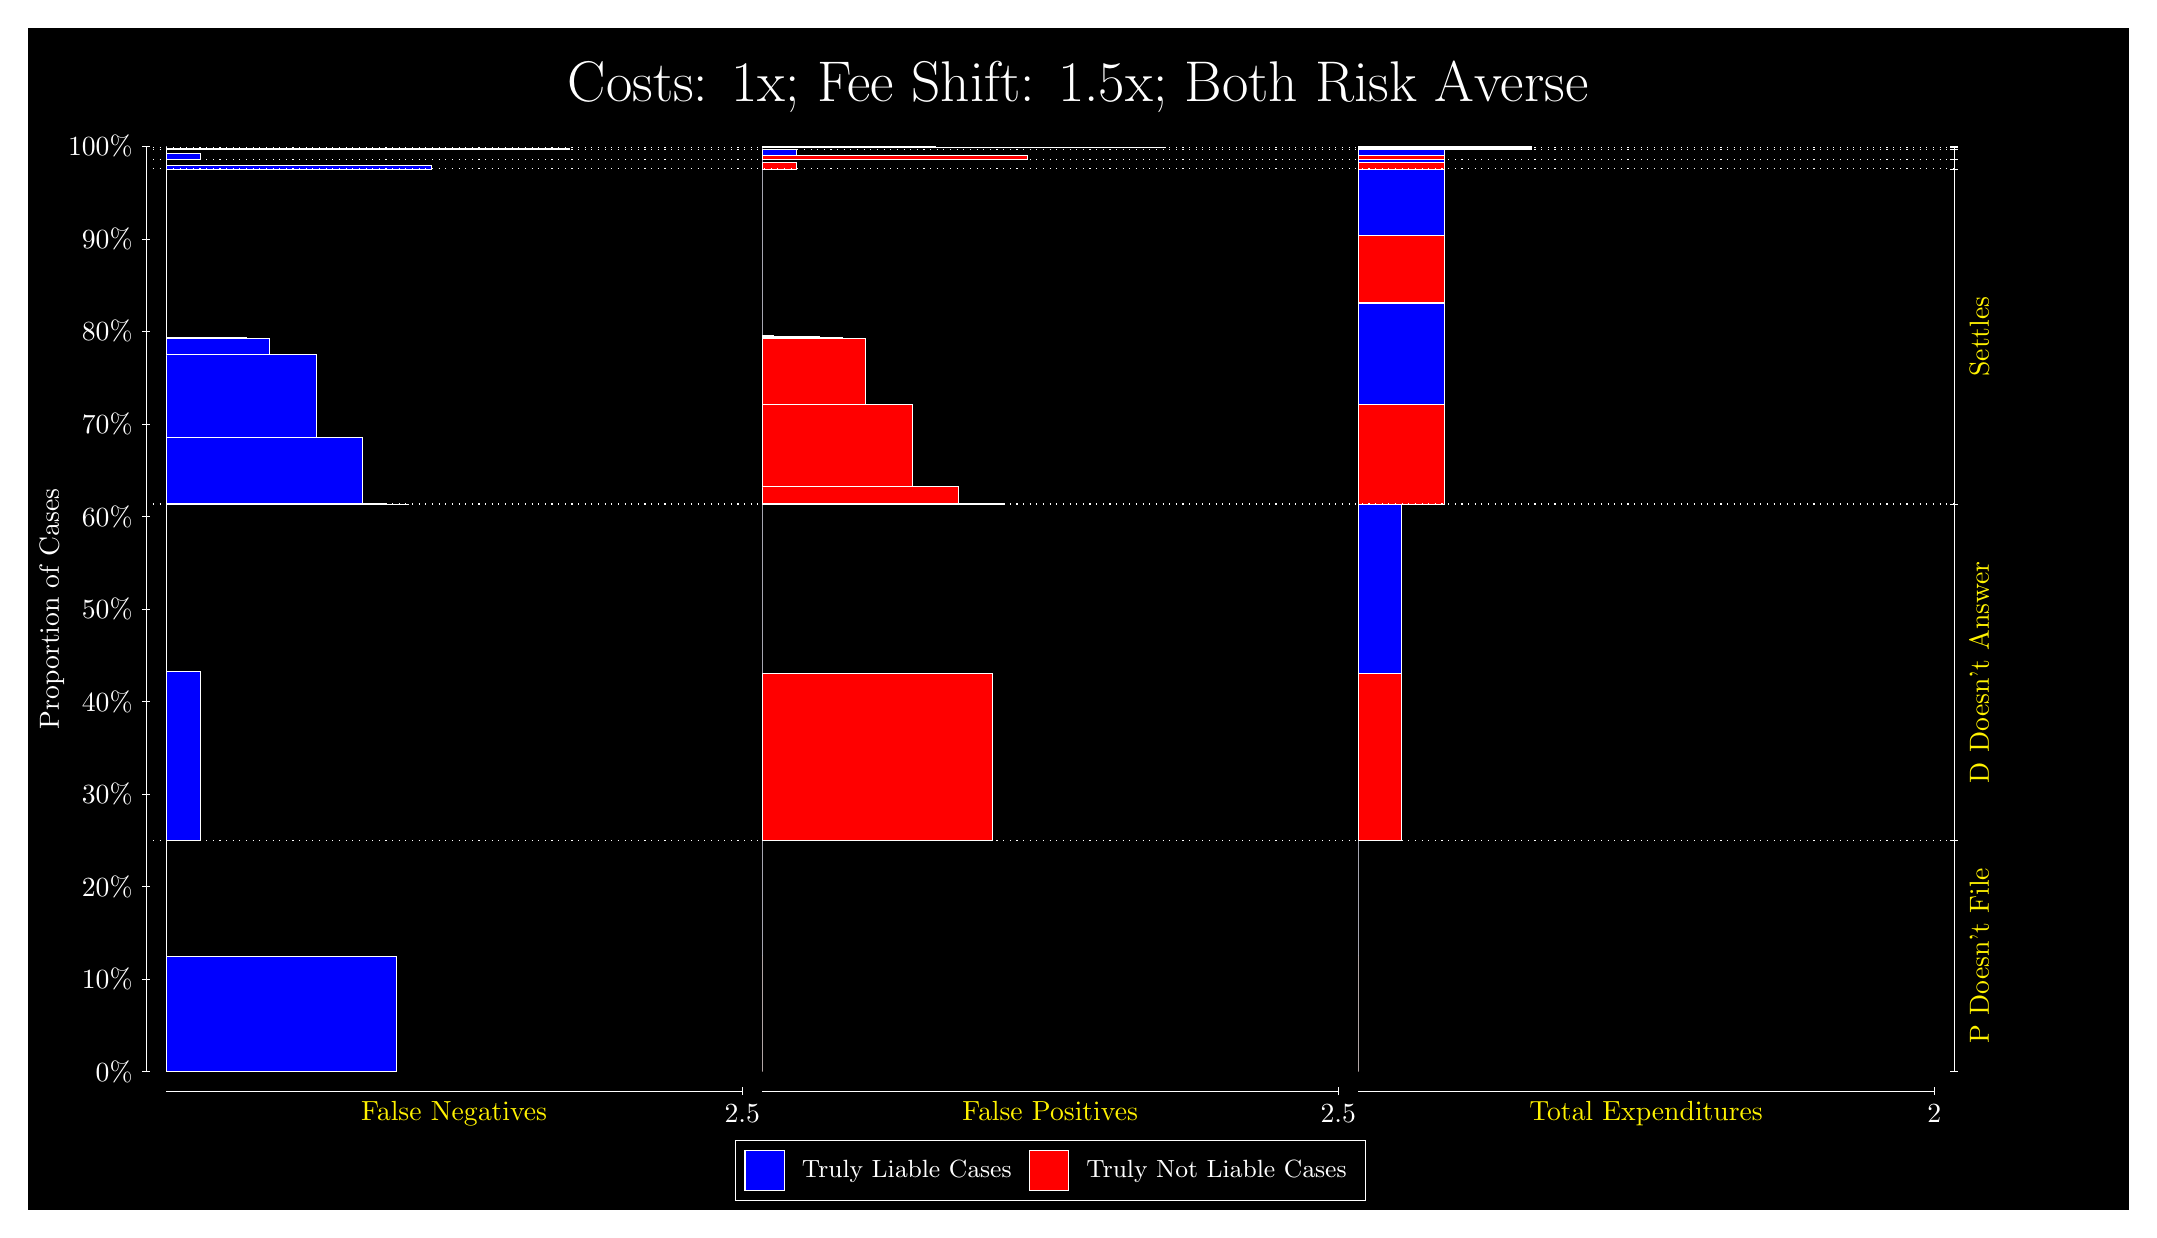
\begin{tikzpicture}
\draw[fill=black] (0,0) rectangle (26.667,15);
\draw[text=white] (0,13.5) rectangle (26.667,15) node[midway] {\huge Costs: 1x; Fee Shift: 1.5x; Both Risk Averse};
\draw[white, very thin] (1.5,1.75) -- (1.5,13.5);
\node[rotate=90, text=white, anchor=center] at (0.3, 7.625) {Proportion of Cases};
\draw[white, very thin] (1.45,1.75) -- (1.55,1.75);
\node[text=white, anchor=east] at (1.45, 1.75) {0\%};
\draw[white, very thin] (1.45,2.925) -- (1.55,2.925);
\node[text=white, anchor=east] at (1.45, 2.925) {10\%};
\draw[white, very thin] (1.45,4.1) -- (1.55,4.1);
\node[text=white, anchor=east] at (1.45, 4.1) {20\%};
\draw[white, very thin] (1.45,5.275) -- (1.55,5.275);
\node[text=white, anchor=east] at (1.45, 5.275) {30\%};
\draw[white, very thin] (1.45,6.45) -- (1.55,6.45);
\node[text=white, anchor=east] at (1.45, 6.45) {40\%};
\draw[white, very thin] (1.45,7.625) -- (1.55,7.625);
\node[text=white, anchor=east] at (1.45, 7.625) {50\%};
\draw[white, very thin] (1.45,8.8) -- (1.55,8.8);
\node[text=white, anchor=east] at (1.45, 8.8) {60\%};
\draw[white, very thin] (1.45,9.975) -- (1.55,9.975);
\node[text=white, anchor=east] at (1.45, 9.975) {70\%};
\draw[white, very thin] (1.45,11.15) -- (1.55,11.15);
\node[text=white, anchor=east] at (1.45, 11.15) {80\%};
\draw[white, very thin] (1.45,12.325) -- (1.55,12.325);
\node[text=white, anchor=east] at (1.45, 12.325) {90\%};
\draw[white, very thin] (1.45,13.5) -- (1.55,13.5);
\node[text=white, anchor=east] at (1.45, 13.5) {100\%};

\draw[white, very thin] (24.457,1.75) -- (24.457,13.5);
\draw[white, very thin] (24.407,1.75) -- (24.507,1.75);
\node[anchor=west] at (24.407, 1.75) {};
\draw[white, very thin] (24.407,4.6875) -- (24.507,4.6875);
\node[anchor=west] at (24.407, 4.6875) {};
\draw[white, very thin] (24.407,8.9573) -- (24.507,8.9573);
\node[anchor=west] at (24.407, 8.9573) {};
\draw[white, very thin] (24.407,13.213) -- (24.507,13.213);
\node[anchor=west] at (24.407, 13.213) {};
\draw[white, very thin] (24.407,13.338) -- (24.507,13.338);
\node[anchor=west] at (24.407, 13.338) {};
\draw[white, very thin] (24.407,13.463) -- (24.507,13.463);
\node[anchor=west] at (24.407, 13.463) {};
\draw[white, very thin] (24.407,13.482) -- (24.507,13.482);
\node[anchor=west] at (24.407, 13.482) {};
\draw[white, very thin] (24.407,13.5) -- (24.507,13.5);
\node[anchor=west] at (24.407, 13.5) {};

\draw[white, very thin, fill=blue] (1.75,1.75) rectangle (4.6775,3.2188);
\draw[white, very thin, fill=red] (1.75,3.2188) rectangle (1.75,4.6875);
\draw[white, very thin, fill=blue] (1.75,4.6875) rectangle (2.1891,6.8389);
\draw[white, very thin, fill=red] (1.75,6.8389) rectangle (1.75,8.9573);
\draw[white, very thin, fill=blue] (1.75,8.9573) rectangle (4.8239,8.9603);
\draw[white, very thin, fill=blue] (1.75,8.9603) rectangle (4.5312,8.9637);
\draw[white, very thin, fill=blue] (1.75,8.9637) rectangle (4.2384,9.8034);
\draw[white, very thin, fill=blue] (1.75,9.8034) rectangle (3.9457,9.8035);
\draw[white, very thin, fill=blue] (1.75,9.8035) rectangle (3.6529,10.853);
\draw[white, very thin, fill=blue] (1.75,10.853) rectangle (3.3602,10.853);
\draw[white, very thin, fill=blue] (1.75,10.853) rectangle (3.0674,11.064);
\draw[white, very thin, fill=blue] (1.75,11.064) rectangle (2.7746,11.069);
\draw[white, very thin, fill=blue] (1.75,11.069) rectangle (2.4819,11.081);
\draw[white, very thin, fill=red] (1.75,11.081) rectangle (1.75,13.213);
\draw[white, very thin, fill=blue] (1.75,13.213) rectangle (5.1167,13.254);
\draw[white, very thin, fill=red] (1.75,13.254) rectangle (1.75,13.338);
\draw[white, very thin, fill=blue] (1.75,13.338) rectangle (2.1891,13.41);
\draw[white, very thin, fill=red] (1.75,13.41) rectangle (1.75,13.463);
\draw[white, very thin, fill=blue] (1.75,13.463) rectangle (6.8732,13.47);
\draw[white, very thin, fill=red] (1.75,13.47) rectangle (1.75,13.482);
\draw[white, very thin, fill=red] (1.75,13.482) rectangle (1.75,13.489);
\draw[white, very thin, fill=blue] (1.75,13.489) rectangle (1.75,13.5);
\draw[white, very thin, fill=red] (9.3189,1.75) rectangle (9.3189,3.2187);
\draw[white, very thin, fill=blue] (9.3189,3.2187) rectangle (9.3189,4.6875);
\draw[white, very thin, fill=red] (9.3189,4.6875) rectangle (12.246,6.8059);
\draw[white, very thin, fill=blue] (9.3189,6.8059) rectangle (9.3189,8.9573);
\draw[white, very thin, fill=red] (9.3189,8.9573) rectangle (12.393,8.9618);
\draw[white, very thin, fill=red] (9.3189,8.9618) rectangle (12.1,8.9671);
\draw[white, very thin, fill=red] (9.3189,8.9671) rectangle (11.807,9.1775);
\draw[white, very thin, fill=red] (9.3189,9.1775) rectangle (11.515,9.1776);
\draw[white, very thin, fill=red] (9.3189,9.1776) rectangle (11.222,10.228);
\draw[white, very thin, fill=red] (9.3189,10.228) rectangle (10.929,10.228);
\draw[white, very thin, fill=red] (9.3189,10.228) rectangle (10.636,11.068);
\draw[white, very thin, fill=red] (9.3189,11.068) rectangle (10.344,11.075);
\draw[white, very thin, fill=red] (9.3189,11.075) rectangle (10.051,11.089);
\draw[white, very thin, fill=blue] (9.3189,11.089) rectangle (9.4652,11.101);
\draw[white, very thin, fill=blue] (9.3189,11.101) rectangle (9.3189,13.213);
\draw[white, very thin, fill=red] (9.3189,13.213) rectangle (9.758,13.297);
\draw[white, very thin, fill=blue] (9.3189,13.297) rectangle (9.3189,13.338);
\draw[white, very thin, fill=red] (9.3189,13.338) rectangle (12.686,13.391);
\draw[white, very thin, fill=blue] (9.3189,13.391) rectangle (9.758,13.463);
\draw[white, very thin, fill=red] (9.3189,13.463) rectangle (9.3189,13.475);
\draw[white, very thin, fill=blue] (9.3189,13.475) rectangle (9.3189,13.482);
\draw[white, very thin, fill=red] (9.3189,13.482) rectangle (14.442,13.489);
\draw[white, very thin, fill=blue] (9.3189,13.489) rectangle (11.515,13.5);
\draw[white, very thin, fill=red] (16.888,1.75) rectangle (16.888,3.2187);
\draw[white, very thin, fill=blue] (16.888,3.2187) rectangle (16.888,4.6875);
\draw[white, very thin, fill=red] (16.888,4.6875) rectangle (17.437,6.8059);
\draw[white, very thin, fill=blue] (16.888,6.8059) rectangle (17.437,8.9573);
\draw[white, very thin, fill=red] (16.888,8.9573) rectangle (17.986,10.228);
\draw[white, very thin, fill=blue] (16.888,10.228) rectangle (17.986,11.506);
\draw[white, very thin, fill=red] (16.888,11.506) rectangle (17.986,11.519);
\draw[white, very thin, fill=blue] (16.888,11.519) rectangle (17.986,11.522);
\draw[white, very thin, fill=red] (16.888,11.522) rectangle (17.986,12.369);
\draw[white, very thin, fill=blue] (16.888,12.369) rectangle (17.986,13.213);
\draw[white, very thin, fill=red] (16.888,13.213) rectangle (17.986,13.297);
\draw[white, very thin, fill=blue] (16.888,13.297) rectangle (17.986,13.338);
\draw[white, very thin, fill=red] (16.888,13.338) rectangle (17.986,13.391);
\draw[white, very thin, fill=blue] (16.888,13.391) rectangle (17.986,13.463);
\draw[white, very thin, fill=red] (16.888,13.463) rectangle (19.083,13.475);
\draw[white, very thin, fill=blue] (16.888,13.475) rectangle (19.083,13.482);
\draw[white, very thin, fill=red] (16.888,13.482) rectangle (19.083,13.489);
\draw[white, very thin, fill=blue] (16.888,13.489) rectangle (19.083,13.5);
\draw[white, dotted] (1.5,4.6875) -- (24.457,4.6875);
\draw[white, dotted] (1.5,8.9573) -- (24.457,8.9573);
\draw[white, dotted] (1.5,13.213) -- (24.457,13.213);
\draw[white, dotted] (1.5,13.338) -- (24.457,13.338);
\draw[white, dotted] (1.5,13.463) -- (24.457,13.463);
\draw[white, dotted] (1.5,13.482) -- (24.457,13.482);
\draw[white, very thin] (1.75,1.5) -- (9.0689,1.5);
\node[text=yellow, anchor=north] at (5.4094, 1.5) {False Negatives};
\draw[white, very thin] (9.0689,1.45) -- (9.0689,1.55);
\node[text=white, anchor=north] at (9.0689, 1.45) {2.5};

\draw[white, very thin] (9.3189,1.5) -- (16.638,1.5);
\node[text=yellow, anchor=north] at (12.978, 1.5) {False Positives};
\draw[white, very thin] (16.638,1.45) -- (16.638,1.55);
\node[text=white, anchor=north] at (16.638, 1.45) {2.5};

\draw[white, very thin] (16.888,1.5) -- (24.207,1.5);
\node[text=yellow, anchor=north] at (20.547, 1.5) {Total Expenditures};
\draw[white, very thin] (24.207,1.45) -- (24.207,1.55);
\node[text=white, anchor=north] at (24.207, 1.45) {2};

\node[text=yellow, centered, rotate=90] at (24.777, 3.2187) {P Doesn't File};
\node[text=yellow, centered, rotate=90] at (24.777, 6.8224) {D Doesn't Answer};
\node[text=yellow, centered, rotate=90] at (24.777, 11.085) {Settles};





\draw (12.978300999999998,1.5) node[draw=none] (baseCoordinate) {};
\begin{scope}[align=center]
        \matrix[scale=0.5, draw=white, below=0.5cm of baseCoordinate, nodes={draw}, column sep=0.1cm]{
            \node[rectangle, draw, minimum width=0.5cm, minimum height=0.5cm, fill=blue] {}; &
            \node[draw=none, font=\small, text=white] (B) {Truly Liable Cases}; &
            \node[rectangle, draw, minimum width=0.5cm, minimum height=0.5cm, fill=red] {}; &
            \node[draw=none, font=\small, text=white] (B) {Truly Not Liable Cases}; \\
            };
\end{scope}

\end{tikzpicture}
\end{document}